% !TEX TS-program = xelatex%

\documentclass[aps, prd
, preprint
%, twocolumn
, nofootinbib 
%, notitlepage
%, superscriptaddress
, longbibliography
]{revtex4-1}
\usepackage{graphicx}
\usepackage[caption=false]{subfig}
\usepackage{mathrsfs}
\usepackage{amsmath,amssymb}
\usepackage{bm}
\usepackage{braket}
\usepackage{listings}
\usepackage{cases}
\usepackage{comment}
\usepackage{soul}
\usepackage{cancel}
\usepackage{cases}
\usepackage[utf8]{inputenc}
\usepackage{url}
\usepackage{longtable}
\usepackage[normalem]{ulem}
\usepackage[colorlinks=true
,urlcolor=blue
,anchorcolor=blue
,citecolor=blue
,filecolor=blue
,linkcolor=blue
,menucolor=blue
%,pagecolor=blue
,linktocpage=true
,pdfproducer=medialab
,pdfa=true
]{hyperref}

%\usepackage{mathpazo}
%\usepackage[no-math]{fontspec}
%\setmainfont{Palatino}
%\setsansfont{Optima}

\newcommand{\dif}[2]{\frac{\mathrm{d} #1}{\mathrm{d} #2}}
\newcommand{\pdif}[2]{\frac{\partial #1}{\partial #2}}
\newcommand{\var}[2]{\frac{\delta #1}{\delta #2}}
\newcommand{\dd}{\mathrm{d}}
\newcommand{\DD}{\mathscr{D}}
\newcommand{\ee}{\mathrm{e}}
\newcommand{\diag}{\mathrm{diag}}
\newcommand{\sgn}{\mathrm{sgn}}
\newcommand{\Mpl}{M_\text{Pl}}
\newcommand{\ns}{n_{{}_\mathrm{S}}}
\newcommand{\cs}{c_{{}_\mathrm{S}}}
\newcommand{\IR}{\text{IR}}
\newcommand{\UV}{\text{UV}}
\renewcommand{\Re}{\mathrm{Re}}
\renewcommand{\Im}{\mathrm{Im}}
\newcommand{\dk}{\frac{\dd^3k}{(2\pi)^3}}
\newcommand{\bbalpha}{{\alpha\!\!\!\alpha}}
\newcommand{\dps}{\displaystyle}
\newcommand{\SIA}{S_\text{IA}}
\newcommand{\eff}{\text{eff}}
\newcommand{\kdx}{\mathbf{k}\cdot\mathbf{x}}
\newcommand{\FP}{\text{FP}}
\newcommand{\cl}{\text{cl}}

\newcommand{\calC}{\mathcal{C}}
\newcommand{\calD}{\mathcal{D}}
\newcommand{\scrD}{\mathscr{D}}
\newcommand{\uf}{\text{f}}
\newcommand{\calg}{\mathcal{g}}
\newcommand{\calH}{\mathcal{H}}
\newcommand{\scrH}{\mathscr{H}}
\newcommand{\uI}{\text{I}}
\newcommand{\ui}{\text{i}}
\newcommand{\calJ}{\mathcal{J}}
\newcommand{\scrJ}{\mathscr{J}}
\newcommand{\calL}{\mathcal{L}}
\newcommand{\scrL}{\mathscr{L}}
\newcommand{\calM}{\mathcal{M}}
\newcommand{\calN}{\mathcal{N}}
\newcommand{\calO}{\mathcal{O}}
\newcommand{\scrO}{\mathscr{O}}
\newcommand{\calP}{\mathcal{P}}
\newcommand{\calR}{\mathcal{R}}
\newcommand{\uR}{\text{R}}
\newcommand{\calV}{\mathcal{V}}

\newcommand{\bae}[1]{\begin{align} #1 \end{align}}
\newcommand{\bce}[1]{\begin{cases} #1 \end{cases}}
\newcommand{\bfe}[4]{
\begin{figure} 
	\centering
	\includegraphics[#1]{#2}
	\caption{#3}
	\label{#4}
\end{figure}}
\newcommand{\bpme}[1]{\begin{pmatrix} #1 \end{pmatrix}}

\newcommand{\Red}[1]{\textcolor{red}{\sffamily #1}}
\newcommand{\Mag}[1]{\textcolor{magenta}{\sffamily #1}}
\newcommand{\Blue}[1]{\textcolor{blue}{\sffamily #1}}
\newcommand{\mathblue}[1]{\textcolor{blue}{#1}}

\allowdisplaybreaks[4]



\begin{document}
\title{Numerical solver of stochastic-$\delta N$ formalism: \texttt{StocDeltaN}}
\date{\today}

\author{Yuichiro Tada}
\email{tada.yuichiro@e.mbox.nagoya-u.ac.jp}
\affiliation{Department of Physics, Nagoya University, Nagoya 464-8602, Japan}

\begin{abstract}
\end{abstract}

\maketitle
%\tableofcontents




\section{Phase space formulation}

\subsection{Basic equations}

Let us consider the following form of the phase space Langevin eq.
\bae{
	\dd\phi^I=f_\phi^I\dd N+g^I_{Qa}\dd W_a, \qquad \dd\pi_I=f_{\pi I}\dd N+g_{PIa}\dd W_a.
}
For a standard choice, the deterministic coefficients are given by
\bae{
	f_\phi^I=G^{IJ}\frac{\pi_J}{H}, \qquad f_{\pi I}=-3\pi_I-\frac{V_I}{H}+\frac{1}{H}\Gamma^K_{IJ}G^{JL}\pi_K\pi_L,
}
with the Hubble parameter calculated by the Friedmann eq.
\bae{
	3\Mpl^2H^2=\frac{1}{2}G^{IJ}\pi_I\pi_J+V.
}
The noise coefficients are determined by the power spectra of linear perturbations. To see the power spectra, it is better to introduce the covariant momenta defined by
\bae{
	\tilde{P}_I=P_I-\Gamma^K_{IJ}\pi_KQ^J.
}
At the leading order in the slow-roll approximation, the correlators between $Q$ and $\tilde{P}$ on the superhorizon scale read
\bae{
	\calP_{QQ}{}^{IJ}\simeq\left(\frac{H}{2\pi}\right)^2G^{IJ}, \qquad \calP_{Q\tilde{P}}{}^I{}_J\simeq\calP_{\tilde{P}\tilde{P}IJ}\simeq0,
}
and therefore those between $Q$ and $P$ are given by
\bae{
	\calP_{QQ}{}^{IJ}\simeq\left(\frac{H}{2\pi}\right)^2G^{IJ}, \qquad \calP_{QP}{}^I{}_J\simeq\Gamma^K_{JL}\pi_K\calP_{QQ}{}^{IL},
	\qquad \calP_{PPIJ}\simeq\Gamma^K_{IL}\Gamma^M_{JN}\pi_K\pi_M\calP_{QQ}{}^{LN}.
}
The noise coefficients are the square-root of these correlators as
\bae{
	g^I_{Qa}\simeq\frac{H}{2\pi}e^I_a, \qquad g_{PIa}\simeq\Gamma^K_{IJ}\pi_Kg^J_{Qa},
}
where $e^I_a$ is a certain choice of the vielbein $e^I_ae^J_a=G^{IJ}$. If one takes account of the mass correction for noise amplitudes,
it would be better to give the vielbein by the adiabatic-entropic decomposition described in Sec.~\ref{sec: Adiabatic-entropic decomposition}.

The corresponding Fokker-Planck (FP) eq. reads
\bae{
	\partial_NP=\calL_{\FP}\cdot P,
}
with the Fokker-Planck operator $\calL_{\FP}$ defined by
\bae{
	\calL_{\FP}\cdot P=-\partial_{\phi^I}(D_{\phi}^IP)-\partial_{\pi_I}(D_{\pi I}P)+\frac{1}{2}\partial_{\phi^I}\partial_{\phi^J}(D_{\phi\phi}{}^{IJ}P)
	+\partial_{\phi^I}\partial_{\pi_J}(D_{\phi\pi}{}^I{}_JP)+\frac{1}{2}\partial_{\pi_I}\partial_{\pi_J}(D_{\pi\pi IJ}P).
}
The coefficients are
\bae{
	\text{It\^o:}& \qquad
	\bce{
		\dps
		D_\phi^I=f_\phi^I, \\
		\dps
		D_{\pi I}=f_{\pi I},
	} \\
	\text{Stratonovich:}& \qquad
	\bce{
		\dps
		D_\phi^I=f_\phi^I+\frac{1}{2}(g^J_{Qa}\partial_{\phi^J}+g_{PJa}\partial_{\pi J})g^I_{Qa}, \\
		D_{\pi I}=f_{\pi I}+\frac{1}{2}(g^J_{Qa}\partial_{\phi^J}+g_{PJa}\partial_{\pi J})g_{PIa}, 
	}
}
and
\bae{
	D_{\phi\phi}{}^{IJ}=g^I_{Qa}g^J_{Qa}=\calP_{QQ}{}^{IJ}, \qquad D_{\phi\pi}{}^I{}_J=g^I_{Qa}g_{PJa}=\calP_{QP}{}^I{}_J, \qquad 
	D_{\pi\pi IJ}=g_{PIa}g_{PJa}=\calP_{PPIJ},
}
both for It\^o and Stratonovich integrals.

For this FP eq., the Vincent's partial differential equation (PDE) is given by
\bae{
	\bce{
		\dps
		\calL_\FP^\dagger\cdot \calM_n=-n\calM_{n-1}, \\ 
		\dps
		\calL_\FP^\dagger\cdot \calC_2=-D_{\phi\phi}{}^{IJ}(\partial_{\phi^I}\calM_1)(\partial_{\phi^J}\calM_1)
		-2D_{\phi\pi}{}^I{}_J(\partial_{\phi^I}\calM_1)(\partial_{\pi_J}\calM_1)-D_{\pi\pi IJ}(\partial_{\pi_I}\calM_1)(\partial_{\pi_J}\calM_1),
	}
}
with $\calM_0=1$ and the absorbing boundary condition $\calM_n|_\text{boundary}=\calC_2|_\text{boundary}=0,\,(n\ge1)$. 
Here $\calM_n(\phi,\pi)=\braket{\calN^n}(\phi,\pi)$, $\calC_2(\phi,\pi)=\braket{\delta\calN^2}(\phi,\pi)$,
and $\calL^\dagger_\FP$ denotes the adjoint FP operator 
\bae{
	\calL^\dagger_\FP=D_\phi^I\partial_{\phi^I}+D_{\pi I}\partial_{\pi_I}+\frac{1}{2}D_{\phi\phi}{}^{IJ}\partial_{\phi^I}\partial_{\phi^J}+D_{\phi\pi}{}^I{}_J\partial_{\phi^I}\partial_{\pi_J}
	+\frac{1}{2}D_{\pi\pi IJ}\partial_{\pi_I}\partial_{\pi_J}.
}



\subsection{Numerical implementation}

\subsubsection{JacobiPDE}

\bfe{width=\hsize}{figs/lattice.pdf}{}{fig: lattice}

In this subsubsection, we describe the numerical algorithm to solve PDE implemented in \texttt{JacobiPDE.hpp}.
To solve PDE numerically, one divides the integration region $\Omega$ into the lattice as schematically indicated in Fig.~\ref{fig: lattice}.
In \texttt{JacobiPDE.hpp}, the Jacobi method is used, where the site value is updated by the nearest eight sites for e.g. 2-dim. case and its own self.

First let us specify the boundary condition. To make use of the $\delta N$ formalism, the surface of the end of inflation should be given by the constant energy slice.
Therefore, with a certain threshold energy $\rho_c$, the boundary condition is set as
\bae{
	\calM_{n(\ge1)}(\phi,\pi)=\calC_2(\phi,\pi)=0, \qquad \text{where $\rho(\phi,\pi)=\rho_c$ (indicated by the blue line in Fig.~\ref{fig: lattice})}.
}
In the discretized lattice case, the site value where $\rho\le\rho_c$ (the blue-shaded region in Fig.~\ref{fig: lattice}) is fixed to zero and not updated during the calculation.

For a hilltop-type inflation model, the integration region $\Omega$ can be surrounded by this end surface $\rho_c$ and the above boundary condition is sufficient.
However, for e.g. a chaotic-type model, the slow-roll inflationary region in general has boundaries between eternal inflationary regions and then the integration region 
$\Omega$ cannot be completely surrounded by absorbing boundaries like as an example Fig.~\ref{fig: lattice}.
In that case, we impose the reflecting condition on these not-EoI (end of inflation) boundaries. 
The Jacobi method requires the nearest sites for each point, so we introduce the imaginary sites one-step outside of $\Omega$.
The field values of these points are determined by those of the reflecting positions which are inside $\Omega$.
The schematic image is indicated in Fig.~\ref{fig: lattice}. Practically, these not-EoI boundaries should be sufficiently far from the interested region
and the boundary condition should not affect the calculation results.

Then we move to the core of the Jacobi method. We label the site point in the $\phi^I$ direction by the small character $i$ of its index $I$ 
(or its fraktur $\mathfrak{i}$ for $\pi_I$). Also only the relevant indices will be explicitly expressed.
Then the first order derivative can be given by one of the following discretizations at leading order.
\bae{
	\partial_{\phi^I}u|_i\simeq\frac{u_{i+1}-u}{h_i}
	\simeq\frac{u-u_{i-1}}{h_{i-1}}
	\simeq\frac{u_{i+1}-u_{i-1}}{h_i+h_{i-1}}.
}
The second derivatives are, depending on if the direction is the same or not, respectively given by
\bae{
	 \bce{
	 	\dps
		\partial_{\phi^I}^2u|_i\simeq2\frac{u_{i+1}h_{i-1}+u_{i-1}h_i-u(h_i+h_{i-1})}{h_ih_{i-1}(h_i+h_{i-1})}, \\
		\dps
		\partial_{\phi^I}\partial_{\phi^J}u|_{ij}\simeq\frac{u_{i+1,j+1}-u_{i+1,j-1}-u_{i-1,j+1}+u_{i-1,j-1}}{(h_i+h_{i-1})(h_j+h_{j-1})}.
	}
}
Regarding the discretization of the first derivative, one recalls that the physically fixed boundary is the EoI surface and field values should be calculated 
from this surface. Therefore the discretization is chosen so that the lower-energy point is used, that is, $u_{i+1}$ if $D^I_\phi>0$ and otherwise $u_{i-1}$ is selected.
Let us label the points where $D_\phi^I>0$ as $i_+$ and $i_-$ for other points (and similarly for $\pi$). Then the adjoint FP operator is discretized as
\bae{
	&\hspace{-20pt}\calL_\FP^\dagger\cdot u \nonumber \\
	\simeq&\sum_{i_+}D_\phi^I\frac{u_{i_++1}-u}{h_{i_+}}+\sum_{j_-}D_\phi^J\frac{u-u_{j_--1}}{h_{j_--1}}
	+\sum_{\mathfrak{i}_+}D_{\pi I}\frac{u_{\mathfrak{i}_++1}-u}{h_{\mathfrak{i}_+}}
	+\sum_{\mathfrak{j}_-}D_{\pi J}\frac{u-u_{\mathfrak{j}_--1}}{h_{\mathfrak{j}_--1}} \nonumber \\
	&+\sum_I\left(D_{\phi\phi}{}^{II}\frac{u_{i+1}h_{i-1}+u_{i-1}h_i-u(h_i+h_{i-1})}{h_ih_{i-1}(h_i+h_{i-1})}
	+D_{\pi\pi II}\frac{u_{\mathfrak{i}+1}h_{\mathfrak{i}-1}+u_{\mathfrak{i}-1}h_\mathfrak{i}-u(h_\mathfrak{i}+h_{\mathfrak{i}-1})}
	{h_\mathfrak{i}h_{\mathfrak{i}-1}(h_\mathfrak{i}+h_{\mathfrak{i}-1})}\right) \nonumber \\
	&+\sum_{I\neq J}\left(\frac{1}{2}D_{\phi\phi}{}^{IJ}\frac{u_{i+1,j+1}-u_{i+1,j-1}-u_{i-1,j+1}+u_{i-1,j-1}}{(h_i+h_{i-1})(h_j+h_{j-1})} \right.\nonumber \\
	&\hspace{20pt}+D_{\phi\pi}{}^I{}_J\frac{u_{i+1,\mathfrak{j}+1}-u_{i+1,\mathfrak{j}-1}-u_{i-1,\mathfrak{j}+1}+u_{i-1,\mathfrak{j}-1}}{(h_i+h_{i-1})(h_\mathfrak{j}+h_{\mathfrak{j}-1})} \nonumber \\
	&\hspace{20pt}\left.+\frac{1}{2}D_{\pi\pi IJ}
	\frac{u_{\mathfrak{i}+1,\mathfrak{j}+1}-u_{\mathfrak{i}+1,\mathfrak{j}-1}-u_{\mathfrak{i}-1,\mathfrak{j}+1}+u_{\mathfrak{i}-1,\mathfrak{j}-1}}
	{(h_\mathfrak{i}+h_{\mathfrak{i}-1})(h_\mathfrak{j}+h_{\mathfrak{j}-1})}\right) \nonumber \\
	=&\left[-\sum_{i_+}\frac{D_\phi^I}{h_{i_+}}+\sum_{j_-}\frac{D_\phi^J}{h_{j_--1}}
	-\sum_{\mathfrak{i}_+}\frac{D_{\pi I}}{h_{\mathfrak{i}_+}}+\sum_{\mathfrak{j}_-}\frac{D_{\pi J}}{h_{\mathfrak{j}_--1}}
	-\sum_I\left(\frac{D_{\phi\phi}{}^{II}}{h_ih_{i-1}}+\frac{D_{\pi\pi II}}{h_\mathfrak{i}h_{\mathfrak{i}-1}}\right)\right]u \nonumber \\
	&-\left[-\sum_{i_+}D_\phi^I\frac{u_{i_++1}}{h_{i_+}}+\sum_{j_-}D_\phi^J\frac{u_{j_--1}}{h_{j_--1}}
	-\sum_{\mathfrak{i}_+}D_{\pi I}\frac{u_{\mathfrak{i}_++1}}{h_{\mathfrak{i}_+}}
	+\sum_{\mathfrak{j}_-}D_{\pi J}\frac{u_{\mathfrak{j}_--1}}{h_{\mathfrak{j}_--1}} \right. \nonumber \\
	&\hspace{20pt}-\sum_I\left(D_{\phi\phi}{}^{II}\frac{u_{i+1}h_{i-1}+u_{i-1}h_i}{h_ih_{i-1}(h_i+h_{i-1})}
	+D_{\pi\pi II}\frac{u_{\mathfrak{i}+1}h_{\mathfrak{i}-1}+u_{\mathfrak{i}-1}h_\mathfrak{i}}
	{h_\mathfrak{i}h_{\mathfrak{i}-1}(h_\mathfrak{i}+h_{\mathfrak{i}-1})}\right) \nonumber \\
	&\hspace{20pt}-\sum_{I\neq J}\left(\frac{1}{2}D_{\phi\phi}{}^{IJ}\frac{u_{i+1,j+1}-u_{i+1,j-1}-u_{i-1,j+1}+u_{i-1,j-1}}{(h_i+h_{i-1})(h_j+h_{j-1})} \right. \nonumber \\
	&\hspace{40pt}+D_{\phi\pi}{}^I{}_J\frac{u_{i+1,\mathfrak{j}+1}-u_{i+1,\mathfrak{j}-1}-u_{i-1,\mathfrak{j}+1}+u_{i-1,\mathfrak{j}-1}}{(h_i+h_{i-1})(h_\mathfrak{j}+h_{\mathfrak{j}-1})}
	\nonumber \\
	&\hspace{40pt}\left.\left.+\frac{1}{2}D_{\pi\pi IJ}
	\frac{u_{\mathfrak{i}+1,\mathfrak{j}+1}-u_{\mathfrak{i}+1,\mathfrak{j}-1}-u_{\mathfrak{i}-1,\mathfrak{j}+1}+u_{\mathfrak{i}-1,\mathfrak{j}-1}}
	{(h_\mathfrak{i}+h_{\mathfrak{i}-1})(h_\mathfrak{j}+h_{\mathfrak{j}-1})}\right)\right] \nonumber \\
	=:&\,Cu-U.
}
Therefore PDE for $\calM_n$ reads
\bae{\label{eq: discrete PDE for fn}
	\calM_n=\left.\frac{1}{C}(-n\calM_{n-1}+U)\right|_{u=\calM_n}.
}
Note that the right side is calculated only by the nearest sites but irrespective of the considered site itself, that is, this equation is explicit.
For $\calC_2$, one discretizes the right side of PDE as well:
\bae{
	&\hspace{-20pt}-D_{\phi\phi}{}^{IJ}(\partial_{\phi^I}v)(\partial_{\phi^J}v)-2D_{\phi\pi}{}^I{}_J(\partial_{\phi^I}v)(\partial_{\pi_J}v)-D_{\pi\pi IJ}(\partial_{\pi_I}v)(\partial_{\pi_J}v) \nonumber \\
	&\simeq-\sum_{IJ}\left[D_{\phi\phi}{}^{IJ}\frac{v_{i+1}-v_{i-1}}{h_i+h_{i-1}}\frac{v_{j+1}-v_{j-1}}{h_j+h_{j-1}} 
	+2D_{\phi\pi}{}^I{}_J\frac{v_{i+1}-v_{i-1}}{h_i+h_{i-1}}\frac{v_{\mathfrak{j}+1}-v_{\mathfrak{j}-1}}{h_\mathfrak{j}+h_{\mathfrak{j}-1}} \right.\nonumber \\
	&\hspace{20pt}\left.+D_{\pi\pi IJ}\frac{v_{\mathfrak{i}+1}-v_{\mathfrak{i}-1}}{h_\mathfrak{i}+h_{\mathfrak{i}-1}}\frac{v_{\mathfrak{j}+1}-v_{\mathfrak{j}-1}}{h_\mathfrak{j}+h_{\mathfrak{j}-1}}
	\right] \nonumber \\
	&=:X.
}
Then PDE reads
\bae{\label{eq: discrete PDE for g2}
	\calC_2=\left.\frac{1}{C}(U+X)\right|_{u=\calC_2,\,v=\calM_1}.
}

Even though these equations are explicit for the considered site, they are still implicit as a whole system and have to be solved algebraically. 
Rather than algebraic transformations, in the Jacobi method, the initial value for each site is given randomly (or maybe given by some analytic form) and then the site value
is repeatedly updated with use of the previous value by following PDE~(\ref{eq: discrete PDE for fn}) or (\ref{eq: discrete PDE for g2}) to find a converged solution.
To estimate the convergence, the following error function is often used.
\bae{
	\text{err}=\frac{|\Delta u|}{|u|},
}
where $\Delta u$ represents the difference between the updated value and the previous one and the absolute value symbol denotes the norm, that is, the square-root of the sum of squares.





\subsubsection{SRK32}

For a numerical solver of stochastic differential equations, we use the R\"o\ss ler's 3-stage order ($2.0,1.0$) strong stochastic Runge-Kutta~\cite{rossler2010runge}.





\subsubsection{StocDeltaN}

\begin{itemize}
\item Explanation of the stochastic-$\delta N$ formalism.
\item User's manual for \texttt{StocDeltaN.hpp}.
\end{itemize}



\subsection{Examples}


\subsection{Adiabatic-entropic decomposition}\label{sec: Adiabatic-entropic decomposition}



\section{Configuration space formulation}

Practically, reducing the phase-space dimension might be the most crucial task from the view point of the computational cost in some cases 
even at the expense of accuracy to some extent. The slow-roll approximation can halve the physical d.o.f. and often gives results practically accurate enough.
In this section, eliminating the d.o.f. of momenta by the slow-roll approximation, we give the configuration space formulation of stochastic-$\delta N$.

In the slow-roll approximation, the Langevin eq. reads
\bae{
	\dd\phi^I=f^I\dd N+g^I_a\dd W_a,
}
with
\bae{
	f^I=-\Mpl^2\frac{V^I}{V}, \qquad g^I_a=\frac{1}{2\pi}\sqrt{\frac{V}{3\Mpl^2}}e^I_a.
}
Then the Fokker-Planck eq. is given by
\bae{
    \partial_NP=\calL_\FP\cdot P=-\partial_I(D^IP)+\frac{1}{2}\partial_I\partial_J(D^{IJ}P),
}
where the coefficients of these equations are related by
\bae{
    D^I=\bce{
        \dps
        f^I, & \text{It\^o} \\[10pt]
        \dps
        f^I+\frac{1}{2}g^J_a\partial_Jg^I_a, & \text{Stratonovich},
    }
    \qquad D^{IJ}=\frac{V}{12\pi^2\Mpl^2}G^{IJ}.
}
Similarly to the full phase-space case, the Vincent's PDE can be obtained as
\bae{
    \bce{
        \dps
        \calL_\FP^\dagger\cdot\calM_n=-n\calM_{n-1}, \\[10pt]
        \dps
        \calL_\FP^\dagger\cdot\calC_2=-D^{IJ}(\partial_I\calM_1)(\partial_J\calM_1),
    }
}
with the adjoint FP operator
\bae{
    \calL_\FP^\dagger=D^I\partial_I+\frac{1}{2}D^{IJ}\partial_I\partial_J,
}
and the same boundary condition.

Numerical discretization can be also done in analogy with the full phase-space formulation as
\bae{
    \calL_\FP^\dagger\cdot u\simeq Cu-U,
}
where
\bae{
    C=&-\sum_{i_+}\frac{D^I}{h_{i_+}}
    +\sum_{j_-}\frac{D^J}{h_{j_--1}}
    -\sum_I\frac{D^{II}}{h_ih_{i-1}}, \\
    U=&-\sum_{i_+}D^I\frac{u_{i_++1}}{h_{i_+}}
    +\sum_{j_-}D^J\frac{u_{j_--1}}{h_{j_--1}}
    -\sum_ID^{II}\frac{u_{i+1}h_{i-1}+u_{i-1}h_i}{h_ih_{i-1}(h_i+h_{i-1})} \nonumber \\
    &-\frac{1}{2}\sum_{I\neq J}D^{IJ}\frac{u_{i+1,j+1}-u_{i+1,j-1}-u_{i-1,j+1}+u_{i-1,j-1}}{(h_i+h_{i-1})(h_j+h_{j-1})},
}
and
\bae{
    -D^{IJ}(\partial_Iv)(\partial_Jv)
    \simeq-\sum_{IJ}D^{IJ}\frac{v_{i+1}-v_{i-1}}{h_i+h_{i-1}}
    \frac{v_{j+1}-v_{j-1}}{h_j+h_{j-1}}=:X,
}
giving the discrete PDE
\bae{
    \calM_n=\left.\frac{1}{C}(-n\calM_{n-1}+U)\right|_{u=\calM_n},
    \qquad \calC_2=\left.\frac{1}{C}(U+X)\right|_{u=\calC_2,\,v=\calM_1}.
}



\subsection{Examples}

\subsubsection{hilltop model}

\begin{figure}
	\centering
	\begin{tabular}{cc}
		\begin{minipage}{0.5\hsize}
			\centering
			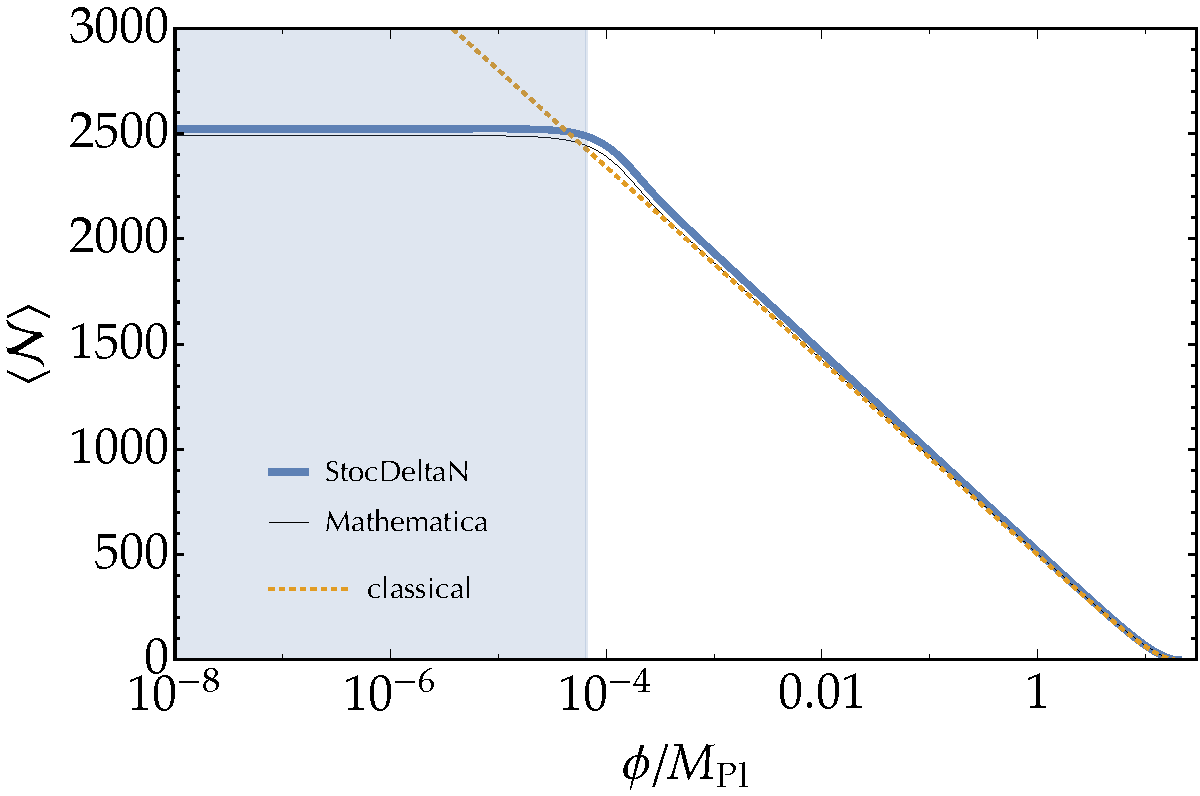
\includegraphics[width=0.9\hsize]{figs/hilltop/N_conf.pdf}
		\end{minipage}
		\begin{minipage}{0.5\hsize}
			\centering
			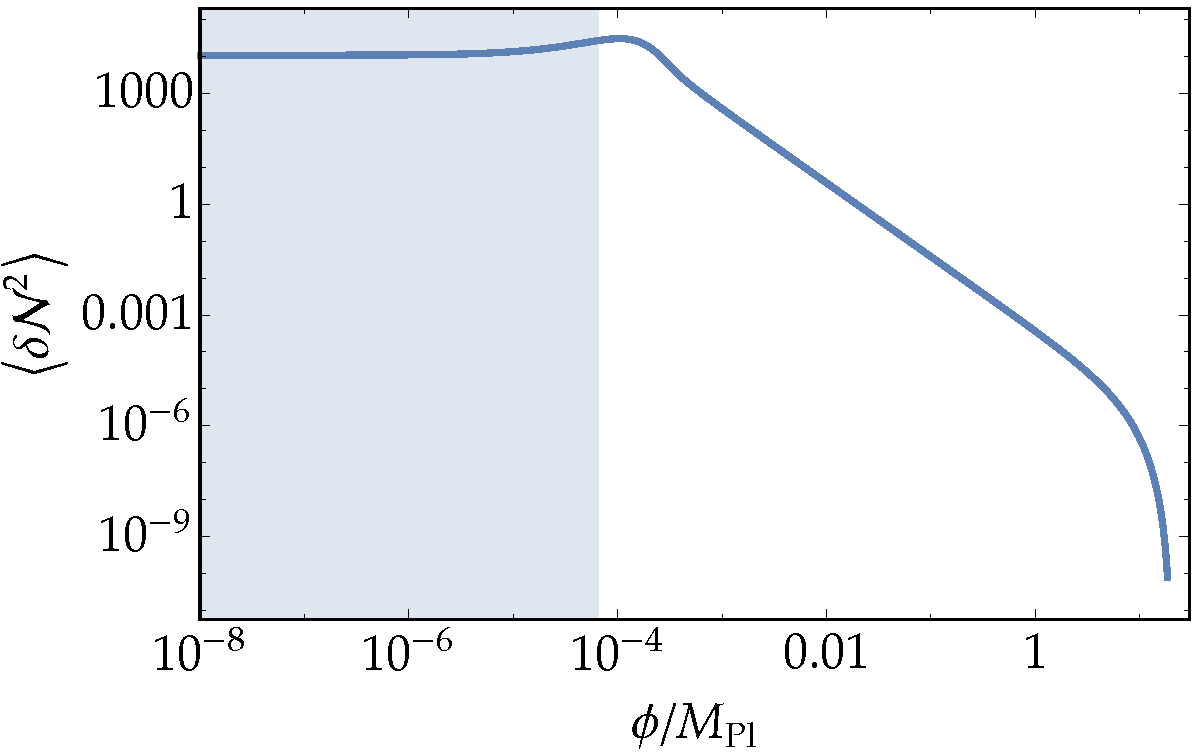
\includegraphics[width=0.9\hsize]{figs/hilltop/dN2_conf.pdf}
		\end{minipage}
	\end{tabular} \\[10pt]
	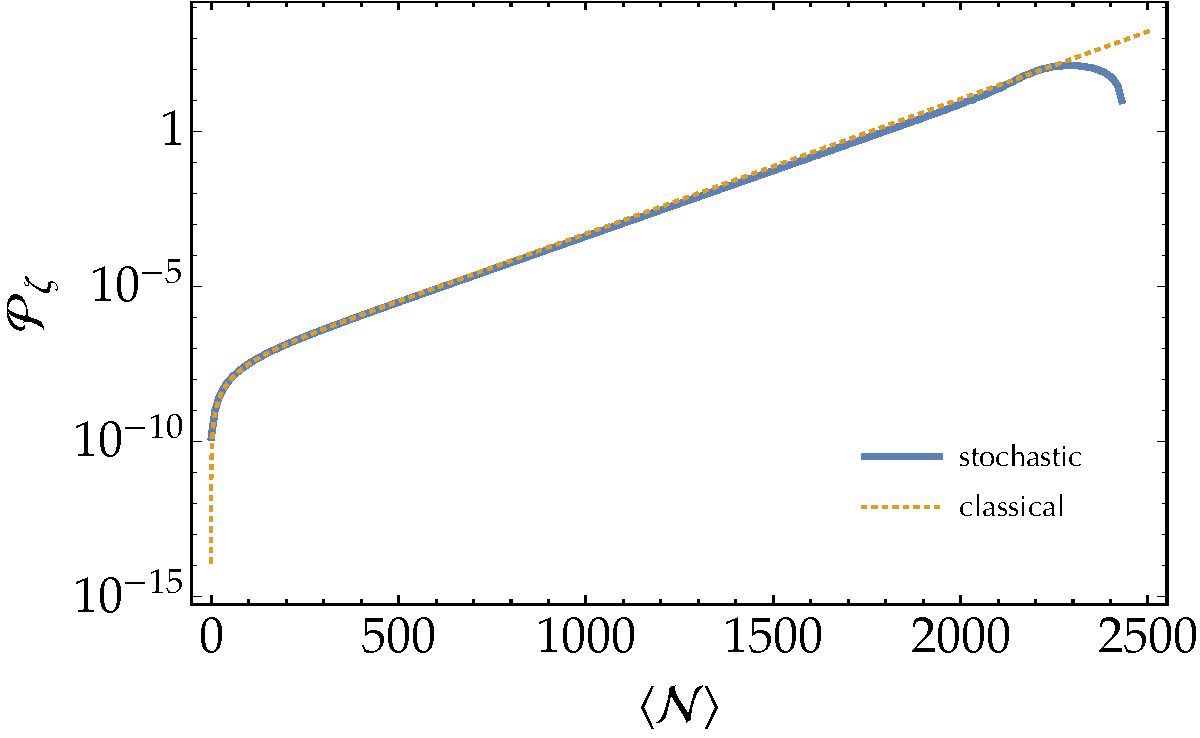
\includegraphics[width=0.5\hsize]{figs/hilltop/Pzeta_conf.pdf}
	\caption{Our numerical results of $\braket{\calN}=\calM_1$, $\braket{\delta\calN^2}=\calC_2$, and $\calP_\zeta=\dd\braket{\delta\calN^2}/\dd\braket{\calN}$ 
	for the hilltop model~(\ref{eq: hilltop V}) are shown by blue thick lines. The end surface is determined by the condition $\epsilon_V=1$. 
	The black thin line represents \texttt{Mathematica}'s numerical integration, while orange dotted lines
	are the classical slow-roll formulae~(\ref{eq: classical slow-roll formulae}). In the shaded region, the stochasticity parameter 
	$\eta_\cl=\frac{1}{24\pi^2\Mpl^4}\left|\frac{V^{\prime\prime}V^2}{{V^\prime}^2}\right|$ becomes larger than unity and the stochastic effect cannot be neglected
	as shown by the deviation between the stochastic calculations (\texttt{StocDeltaN} or \texttt{Mathematica}) and the classical ones.}
	\label{figs: hilltop_conf}
\end{figure}

Let us first consider the hilltop model which is already studied by Vincent's original paper~\cite{Vennin:2015hra} and a good example to see the stochastic effect.
The potential is given by
\bae{\label{eq: hilltop V}
	V=\Lambda^4\left[1-\left(\frac{\phi}{\mu}\right)^2\right], \qquad \Lambda=10^{-2}\Mpl, \qquad \mu=20\Mpl.
}
The results are shown in Fig.~\ref{figs: hilltop_conf}. In single-field models, the Vincent's PDE reduces to ordinary differential equations (ODE) and at least $\calM_1$ can be solved 
easily even in \texttt{Mathematica} ($\calC_2$ requires the result of $\calM_1$ and is much heavier), then we compare \texttt{Mathematica}'s result with that of our numerical code,
showing they are consistent. 
When the stochasticity parameter $\eta_\cl=\frac{1}{24\pi^2\Mpl^4}\left|\frac{V^{\prime\prime}V^2}{{V^\prime}^2}\right|$ is large, 
the stochastic sweeping effect reduces both the mean e-folds and its perturbation from the classical slow-roll predictions given by
\bae{\label{eq: classical slow-roll formulae}
	N_\cl=\int^\phi_{\phi_\uf}\frac{\dd\phi^\prime}{\Mpl}\frac{1}{\sqrt{2\epsilon_V}}, \qquad \calP_\zeta=\frac{1}{24\pi^2\Mpl^4}\frac{V}{\epsilon_V}, 
	\qquad \epsilon_V=\frac{\Mpl^2}{2}\left(\frac{V^\prime}{V}\right)^2.
}
In particular, the results show that the mean e-folds cannot exceed around 2500 by the sweeping effect and then the power spectrum rapidly reduces around that scale 
(though the curvature perturbations largely exceed unity around this scale and the validity of the stochastic-$\delta N$ formalism might be doubtful).





\subsubsection{inflection model}

\begin{figure}
	\centering
	\begin{tabular}{cc}
		\begin{minipage}{0.5\hsize}
			\centering
			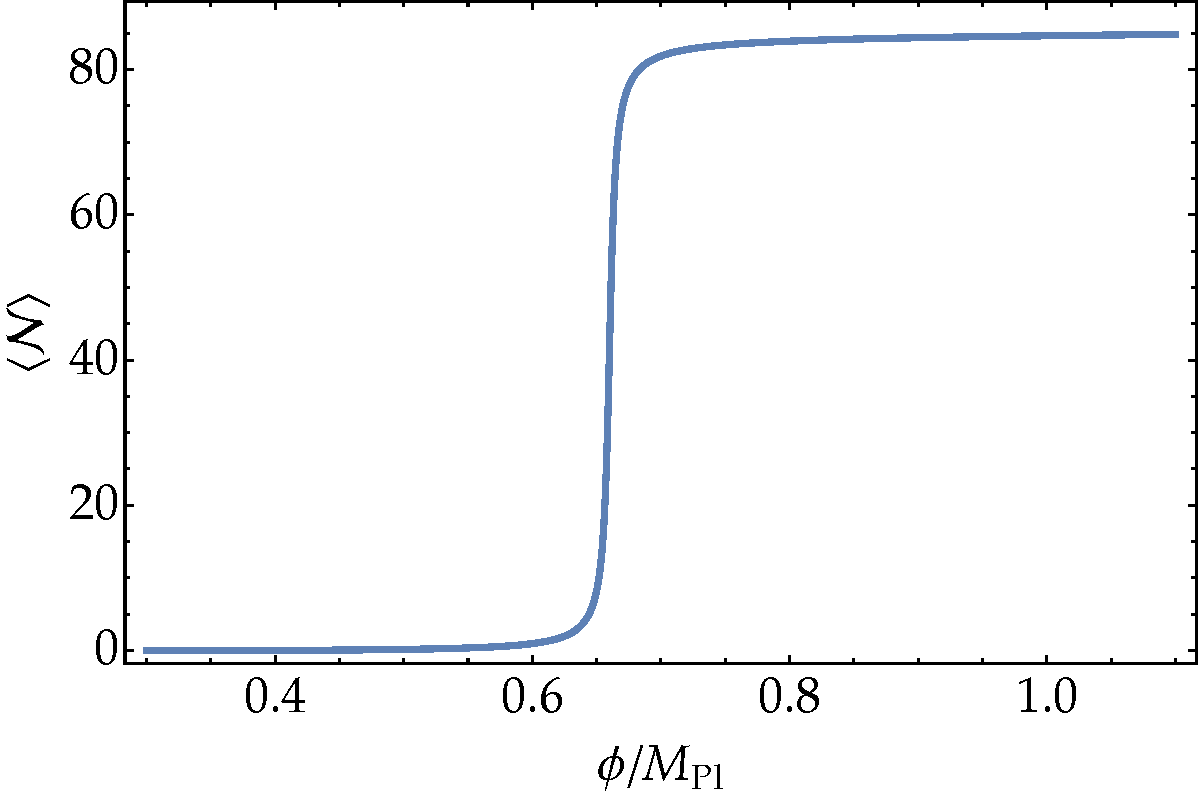
\includegraphics[width=0.9\hsize]{figs/inflection/N_conf.pdf}
		\end{minipage}
		\begin{minipage}{0.5\hsize}
			\centering
			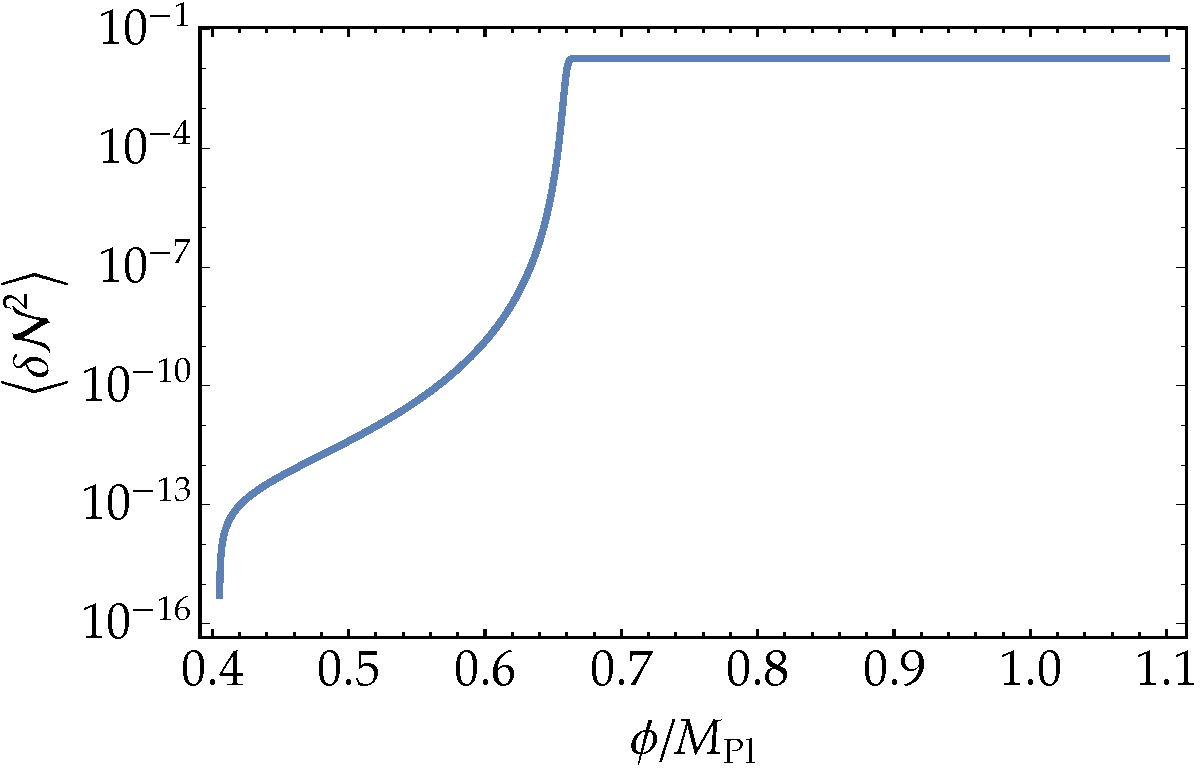
\includegraphics[width=0.9\hsize]{figs/inflection/dN2_conf.pdf}
		\end{minipage}
	\end{tabular} \\[10pt]
	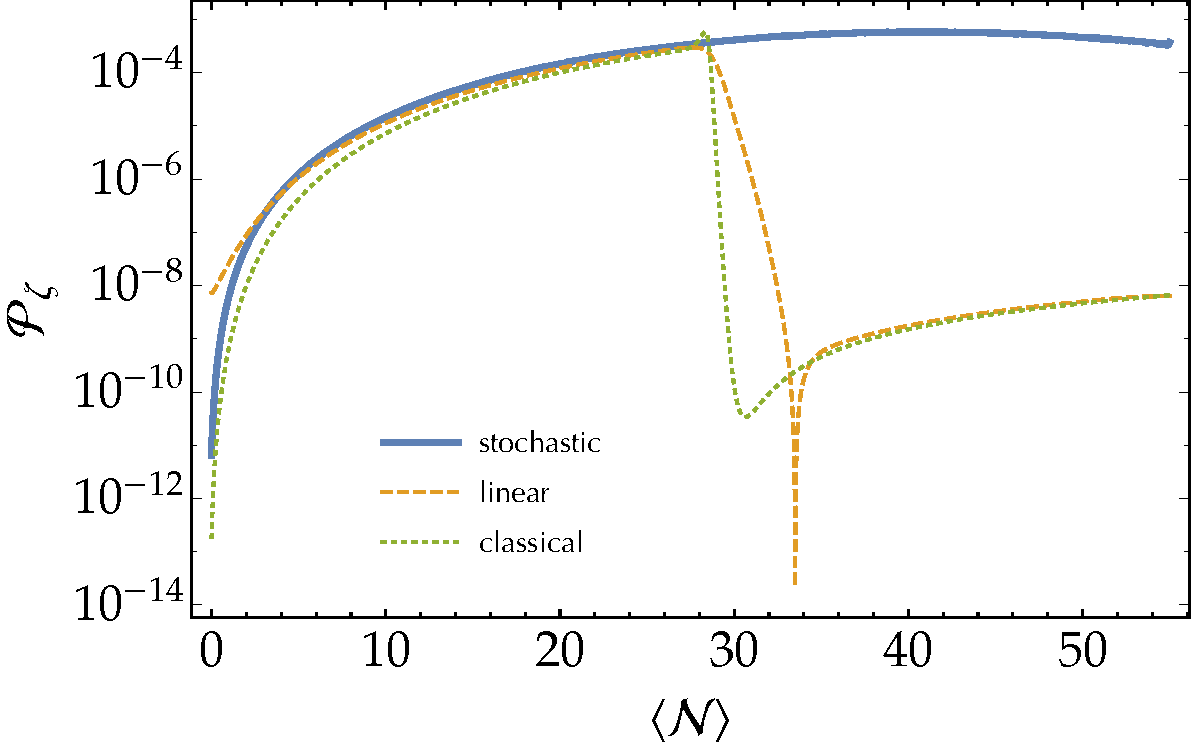
\includegraphics[width=0.5\hsize]{figs/inflection/Pzeta_conf.pdf}
	\caption{Results for the inflection model~(\ref{eq: inflection V}). The end surface is $\rho_\uf=3\times(1.9\times10^{-5})^2\Mpl^4$. 
	The orange dashed line represents the result in the full (Mukhanov-Sasaki) linear perturbation theory,
	while the green dotted line corresponds with the classical slow-roll approximation~(\ref{eq: classical slow-roll formulae}) though the dynamics of $\epsilon_V$ itself is
	calculated without the slow-roll approximation.}
	\label{figs: inflection_conf}
\end{figure}

Let us see the model beyond the slow-roll approximation, that is, the ultra-slow-roll inflection model~\cite{Garcia-Bellido:2017mdw,Ezquiaga:2018gbw}:
\bae{\label{eq: inflection V}
	V=\frac{V_0}{12}\frac{6m^2\phi^2-4\alpha\phi^3+3\lambda\phi^4}{(1+\xi\phi^2)^2},
}
where the parameters are chosen so that the potential has very flat inflection point at the critical point $\phi_c=0.66$ as,
\bae{
	V_0=10^{-7}, \qquad \lambda=1, \qquad \xi=2.3, \qquad \alpha=\frac{6\lambda\phi_c}{3+\xi^2\phi_c^4}, \qquad m^2=\frac{\lambda\phi_c^2(3+\xi\phi_c^2)}{3+\xi^2\phi_c^4},
}
in the Planck unit $\Mpl=1$.

As studied in Ref.~\cite{Garcia-Bellido:2017mdw}, while the dynamics is well described by the slow-roll attractor solution sufficiently before the critical point,
the potential tilt rapidly reduces around $\phi_c$ and the inflaton momentum estimated by the slow-roll approximation becomes much smaller than the true value,
meaning the violation of the slow-roll approximation known as the ultra-slow-roll case.

\texttt{StocDeltaN}'s results are summarized in Fig.~\ref{figs: inflection_conf}, compared with those in the textbook approaches.
Since we employ the slow-roll EoM in this section, the stochastic-$\delta N$ formalism cannot follow the rapid change of the potential tilt but instead
shows a broad peak. That is, the full phase-space formulation is required in this case.




\subsubsection{double mass-term model}

\begin{figure}
	\centering
	\begin{tabular}{cc}
		\begin{minipage}{0.5\hsize}
			\centering
			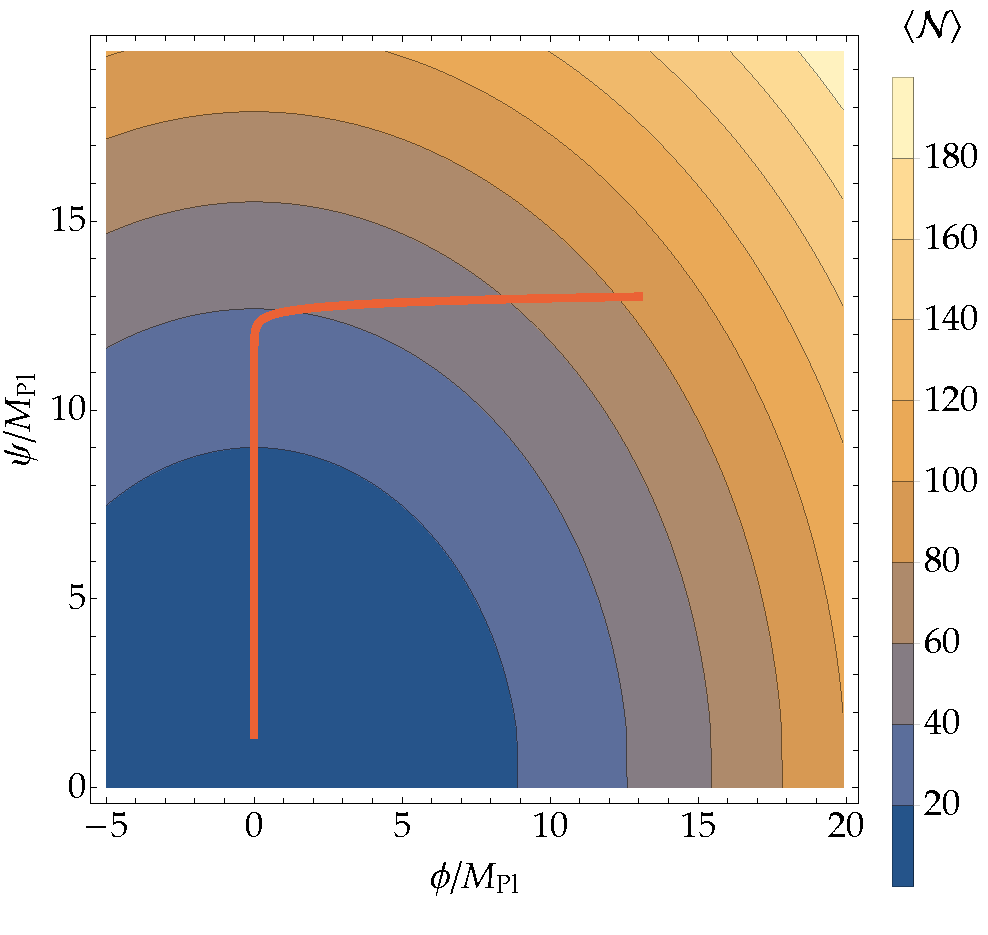
\includegraphics[width=0.9\hsize]{figs/double_chaotic/N_conf.pdf}
		\end{minipage}
		\begin{minipage}{0.5\hsize}
			\centering
			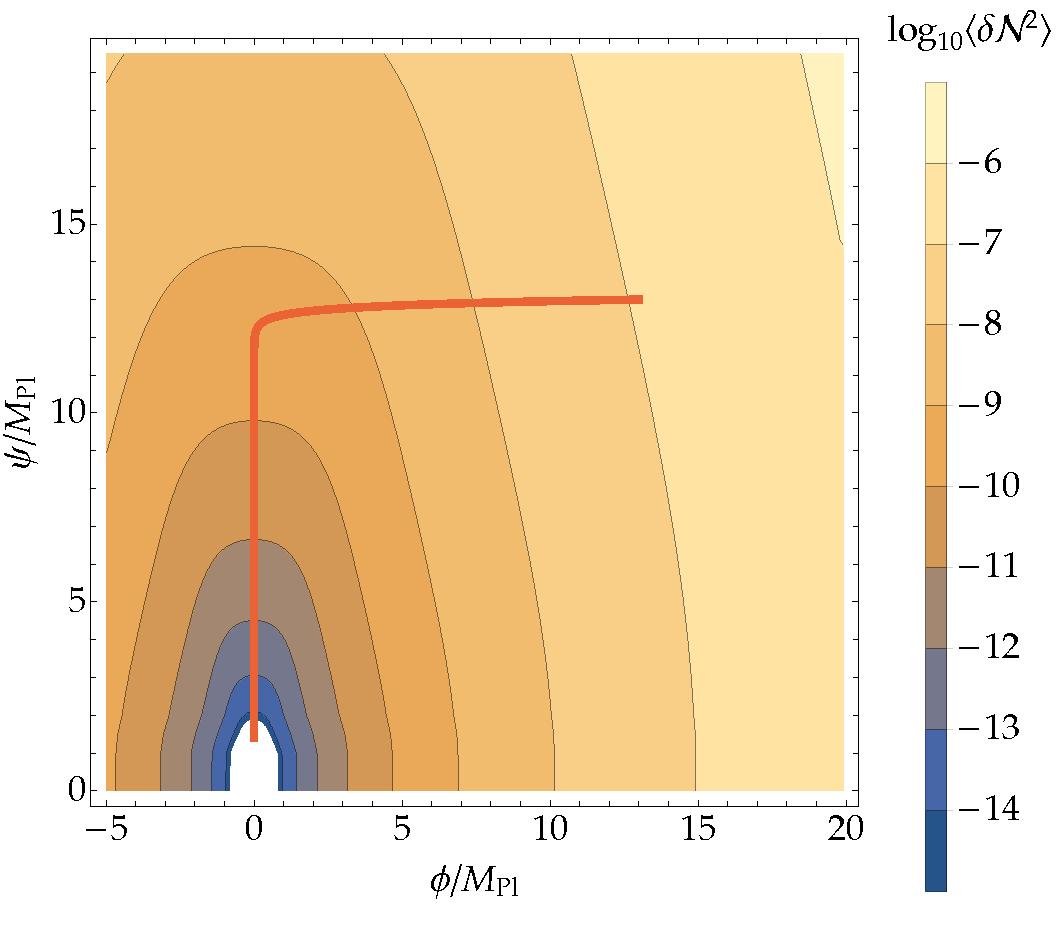
\includegraphics[width=0.9\hsize]{figs/double_chaotic/dN2_conf.pdf}
		\end{minipage}
	\end{tabular} \\[10pt]
	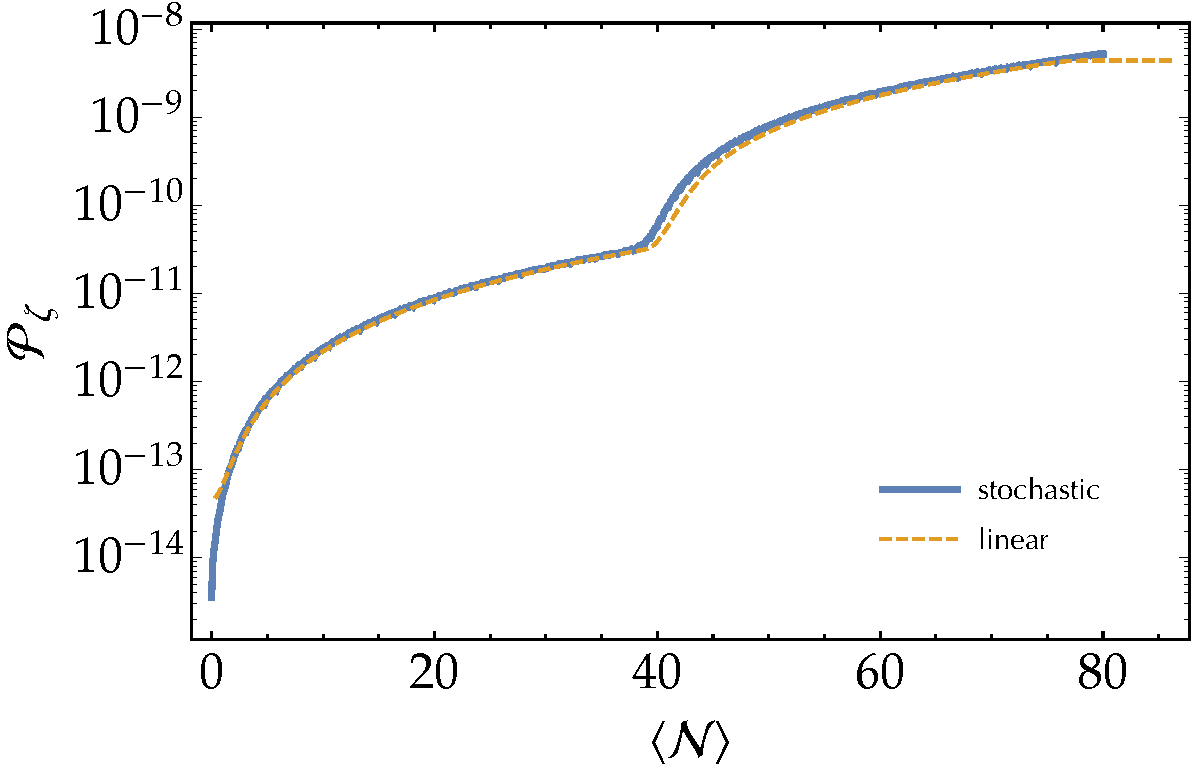
\includegraphics[width=0.5\hsize]{figs/double_chaotic/Pzeta_conf.pdf}
	\caption{Double mass-term model described by (\ref{eq: double chaotic V}). The end surface is $\rho_\uf=m_\psi^2$.
	The red lines in the upper two figures shows one sample trajectory started from $\phi_\ui=\psi_\ui=13\Mpl$. The power spectrum of curvature perturbations
	shown in the lower figure is calculated around such trajectories.}
	\label{figs: double_chaotic_conf}
\end{figure}

As a first simple example of multi-field models, let us here consider the double mass-term model whose potential is given by
\bae{\label{eq: double chaotic V}
	V=\frac{1}{2}M^2\phi^2+\frac{1}{2}m^2\psi^2, \qquad M=9m=10^{-5}\Mpl,
}
with the canonical field-space metric $G_{IJ}=\diag(1,1)$. The result is shown in Fig.~\ref{figs: double_chaotic_conf}.
In this setup, the stochasticity of the considered region is small and the stochastic-$\delta N$ formalism well reproduces
the results of the linear perturbation (Mukhanov-Sasaki) theory 
except for slight differences around the turning point expected to be due to the slow-roll approximation.
This example indicates that our numerical code is useful even for models where the stochastic effect is not significant.



\subsubsection{hybrid model}

\begin{figure}
	\centering
	\begin{tabular}{cc}
		\begin{minipage}{0.5\hsize}
			\centering
			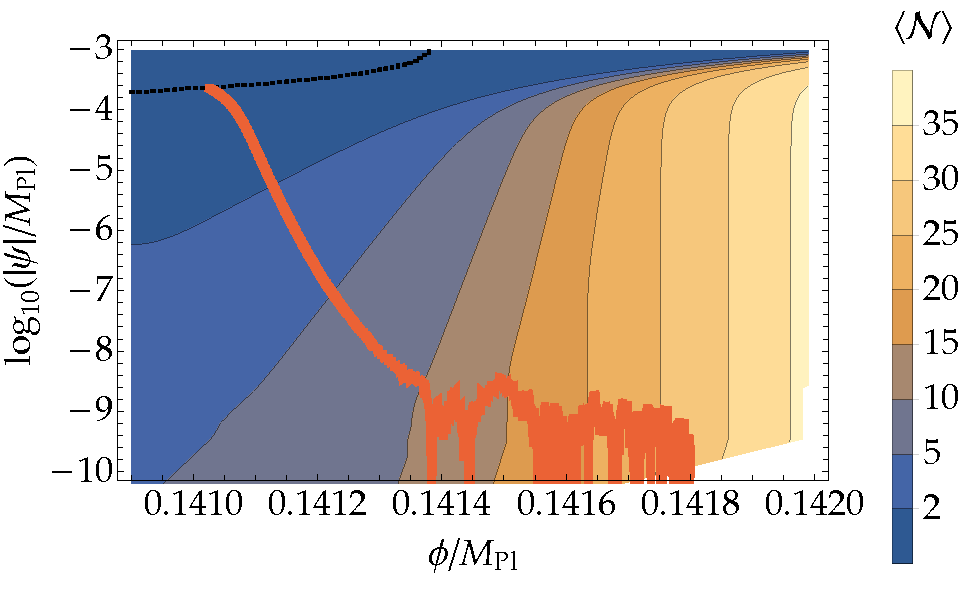
\includegraphics[width=0.9\hsize]{figs/hybrid/N_conf.pdf}
		\end{minipage}
		\begin{minipage}{0.5\hsize}
			\centering
			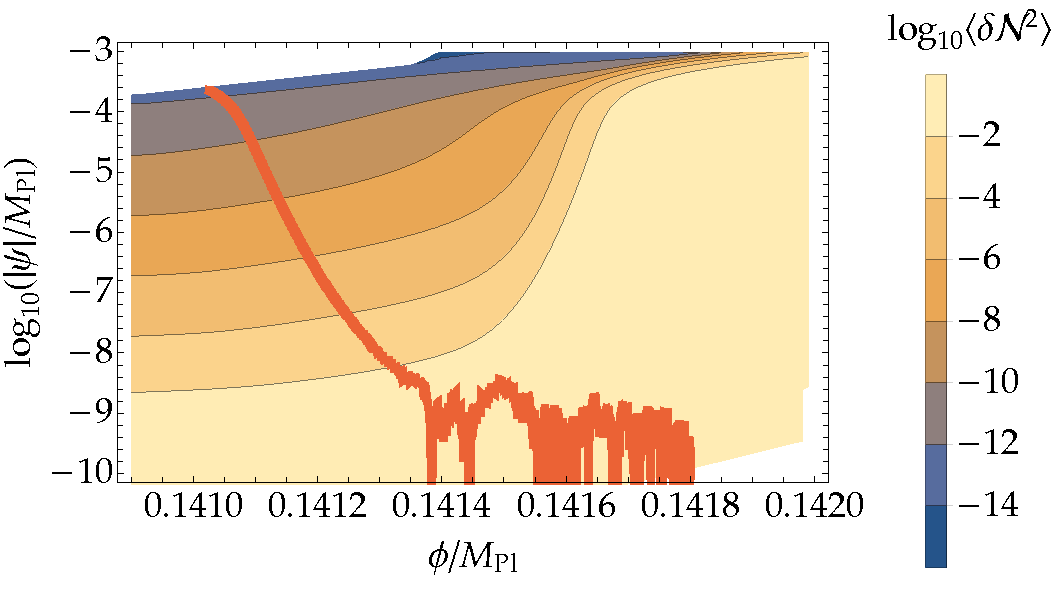
\includegraphics[width=0.9\hsize]{figs/hybrid/dN2_conf.pdf}
		\end{minipage}
	\end{tabular} \\[10pt]
	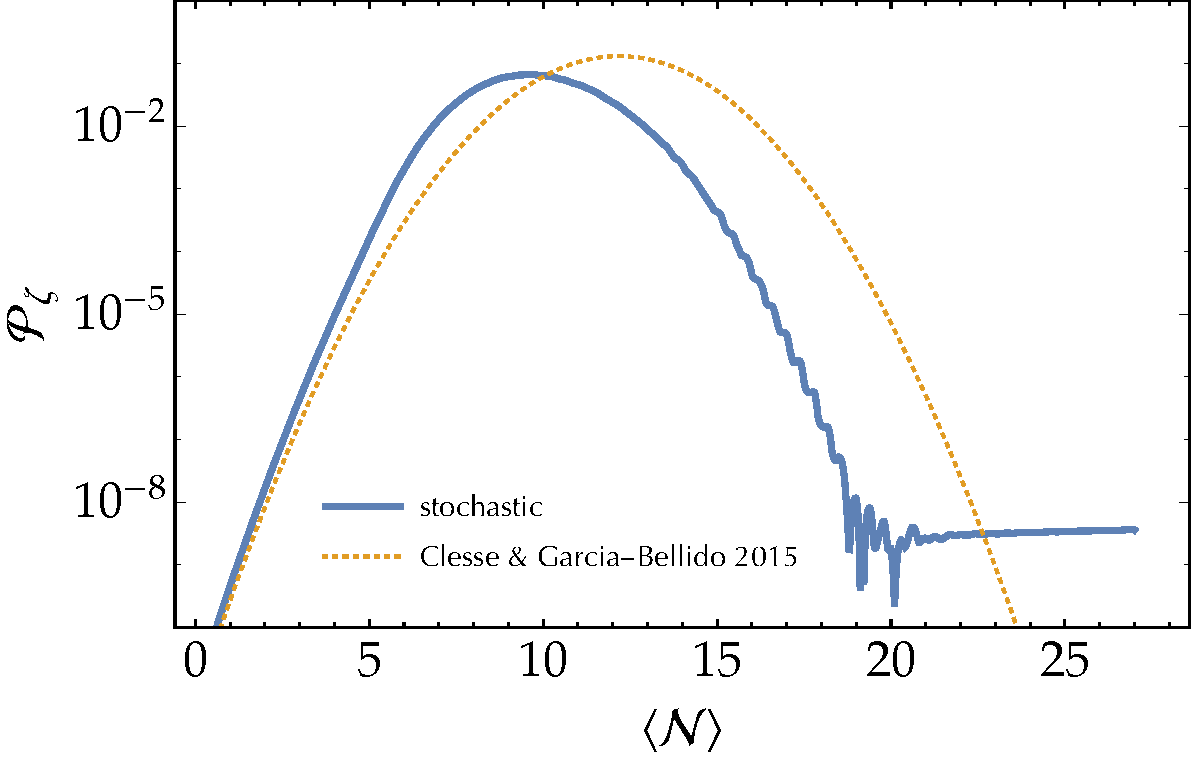
\includegraphics[width=0.5\hsize]{figs/hybrid/Pzeta_conf.pdf}
	\caption{Hybrid inflation model (\ref{eq: hybrid V}). The black dotted line in the top-left figure represents the end surface $\rho_\uf=2.074038\times10^{-16}\Mpl^4$.
	The orange dotted line in the lower figure represents the semi-classical formula (\ref{eq: CG formula}) by Clesse \& Garc\'ia-Bellido~\cite{Clesse:2015wea}.}
	\label{figs: hybrid_conf}
\end{figure}

The true powerfulness of our code becomes clear for models where the stochastic correction is necessary, e.g. the critical point of hybrid inflation~\cite{Kawasaki:2015ppx}:
\bae{\label{eq: hybrid V}
	V=\Lambda^4\left[\left(1-\frac{\psi^2}{M^2}\right)^2+2\frac{\phi^2\psi^2}{\phi_c^2M^2}+\frac{\phi-\phi_c}{\mu_1}-\frac{(\phi-\phi_c)^2}{\mu_2^2}\right],
}
where
\bae{
	M=0.1, \qquad \phi_c=0.1\sqrt{2}, \qquad \mu_1=\frac{50}{M^2\phi_c}, \qquad \mu_2=11, \qquad \Lambda=2.189\times10^{-9}\times\frac{12\pi^2}{\mu_1^2},
}
in the Planck unit $\Mpl=1$. Clesse \& Garc\'ia-Bellido derived a semi-classical formula for this model as~\cite{Clesse:2015wea}
\bae{\label{eq: CG formula}
	\calP_{\zeta,\text{CG}}(k)=\frac{\Lambda^4M^2\phi_c\mu_1}{192\pi^2\Mpl^2\chi_2\psi_k^2},
}
where
\bae{
	\psi_k=\psi_0\ee^{\chi_k}, \qquad \chi_k=\frac{4\phi_c\mu_1\xi_k^2}{M^2}, \qquad \xi_k=\frac{(N_k-N_\text{water})\Mpl^2}{\mu_1\phi_c},
}
for the mode $k=k_\uf\ee^{-N_k}$ with
\bae{
	\psi_0&=\left(\frac{\sqrt{2}\Lambda^4M\phi_c^{1/2}\mu_1^{1/2}}{96\pi^{3/2}\Mpl^4}\right)^{1/2}, \qquad 
	N_\text{water}=\left(\frac{\sqrt{\chi_2}}{2}+\frac{1}{4\sqrt{\chi_2}}\right)\frac{M\phi_c^{1/2}\mu_1^{1/2}}{\Mpl^2}, \nonumber \\
	\chi_2&=\log\left(\frac{\phi_c^{1/2}M}{2\mu_1^{1/2}\psi_0}\right).
}
As the previous calculation in Ref.~\cite{Kawasaki:2015ppx}, the stochastic-$\delta N$ formalism gives results qualitatively consistent with this formula, 
shown in Fig.~\ref{figs: hybrid_conf}. Particularly, our \texttt{StocDeltaN} reproduces not only the peak spectrum but also the flat one at the valley phase 
$\braket{\calN}\gtrsim20$, while the previous calculation is dominated by large sampling noises.






\subsubsection{GeoDesI}





%\acknowledgments





%\appendix







\bibliography{main}
\end{document}
